\documentclass[10pt,a4paper]{article}
\usepackage[T1]{fontenc}
\usepackage[utf8]{inputenc}
\usepackage[margin=22mm]{geometry}
\usepackage{lmodern}
\usepackage{amsmath,booktabs,array,graphicx,needspace}
\usepackage[hyphens]{url}
\usepackage[hidelinks]{hyperref}
\setlength{\parskip}{3pt}
\setlength{\emergencystretch}{2em}
\clubpenalty=10000
\widowpenalty=10000
\hypersetup{pdftitle={Resource-Efficient Local Language Models for Agricultural Tasks: A 9B--27B Comparison with Deterministic Tools},pdfauthor={Antoniy Sarychev; Denis Shesternin},pdfsubject={Working empirical draft; final author consent and license pending}}
\begin{document}
\begin{center}\bfseries Resource-Efficient Local Language Models for Agricultural Tasks: A 9B--27B Comparison with Deterministic Tools\end{center}

Antoniy Sarychev, Denis Shesternin


Russian State Agrarian University --- Moscow Timiryazev Agricultural Academy, Moscow, Russia


Working empirical draft, 4 October 2026. Prepared for editorial review; final approval by both authors and manuscript license remain pending. The Russian and English texts are versions of one study.


\section*{Abstract}

We examine the quality, latency and memory tradeoff of two practical local language-model configurations on one consumer PC, and distinguish tool declaration from completed deterministic execution. On the public development split of MERA ruTXTAgroBench, Qwen3.5-9B Q8\_0 and Qwen3.8-27B UD-Q4\_K\_M attain strict option-set exact match of 141/289 and 150/289, respectively; four original references remain unresolved. A separate native-transport TELEMETRY40 run is scored retrospectively: exact match is 22/39 versus 24/39, with median request latency 0.269 versus 1.434 seconds and sampled whole-GPU peaks of 11,471 versus 13,287 MiB. Exact input texts and recorded weight hashes agree with the historical run, but schema, seed, checkpoint caching and GPU placement differ, and some choices change. We therefore keep full-split quality and native telemetry separate. The live constructed calculation study obtains full correctness of 7/27 versus 18/27 for Qwen9 without/with tools and 15/27 versus 25/27 for Qwen27; each tool arm achieves 16/16 numeric answers, while clarification errors remain. These development observations support a bounded configuration tradeoff, without establishing equivalence, a causal parameter-count effect, or the safety of agricultural advice.


Keywords: local language models; agricultural benchmarks; resource efficiency; deterministic computation; tool execution; reproducibility.


\section{Research problem and contribution}

Local agricultural assistants face both knowledge questions and precisely specified calculations. The first may require domain knowledge; the second can often be checked against an explicit formula and units. A small local model may reduce latency and occupied memory, yet a plausible output or a correctly named tool can still conceal an incorrect answer. Deployment decisions therefore require evidence about the complete evaluated configuration and the executed computation.


Our primary question is the observed quality--resource tradeoff between Qwen3.5-9B and Qwen3.8-27B on a consumer PC. The second asks how model-only calculation compares with actual allowlisted deterministic execution. Cloud escalation is a supplementary question that can have a negative or inconclusive answer. We study practical configurations that differ in model generation, size, quantization and placement. This design does not isolate the causal effect of parameter count.


The contribution is an auditable development case study: a preserved agricultural benchmark comparison, a retrospective compatibility check linking saved predictions to telemetry, and a separately identified calculation experiment. No new hidden MERA TEST was generated or submitted. We retain the 9B configuration as the focal practical option and the 27B configuration as a stronger observed-quality reference, without defining a post-hoc acceptable quality loss.


\section{Related literature}

FrugalGPT, AutoMix, Hybrid LLM, RouteLLM and the unified routing framework formalize model selection and escalation \cite{ref1,ref2,ref3,ref4,ref5}. RouterBench separates cached-output comparisons from the behavior and cost of a deployed router \cite{ref6}. Their methods motivate measuring the resources of the actual serving configuration; their published gains do not establish gains for our models, data or hardware. Our saved-output routing analyses remain exploratory replay.


Semantic Entropy Probes and the abstention survey show that reliability requires a defined uncertainty or refusal criterion \cite{ref7,ref8}. An output confidence field, lexical support check or grammatical JSON object alone cannot establish correctness. In this study, format compliance, transport completion, option-set quality and input clarification are reported separately.


PLLaMa, AgriGPT and AgroLLM investigate agricultural adaptation or knowledge transfer \cite{ref9,ref10,ref11}. AgriAgent and AgroTools address agricultural planning and tool orchestration \cite{ref12,ref13}; thus agriculture plus tools is already an established research direction. Our narrower comparison concerns local resources and the difference between a declared and an executed calculation. tau-bench evaluates completed interaction goals, while ToolACE studies function-calling data and validation \cite{ref14,ref15}. These distinctions inform our complete-answer rather than tool-name-only scoring.


Efficient architectures and quantization also require careful identity control. The BitNet work describes native low-bit models, and the Gemma 4 report covers dense and mixture-of-experts architectures \cite{ref16,ref17}. Neither supplies measurements for the third-party GGUF configurations in this paper. AgXQA offers a different agricultural question-answering setting \cite{ref18}, used in historical HOME experiments rather than as interchangeable MERA data. For computation we use the foundational FAO-56 equations and units \cite{ref19}, separately from recent AI references.


\section{Data, configuration and analysis}

\subsection*{Separate evidence blocks}

MERA ruTXTAgroBench contains 2,935 Russian multiple-choice questions across ten agricultural disciplines, including 293 public DEV items. Its creators describe agricultural-expert authorship, professional editing and checking by three experts. This is attributed methodology, not our independent verification of every key or farm-level applicability. We use public DEV under the documented restrictions; questions, gold and unrestricted benchmark logs remain outside the editorial package and software release.


The initial balanced DEV60 screen is contained in DEV293. Model selection and previous prompt/scorer inspection therefore affect the full-split results. TELEMETRY40 selects four positions per discipline without inspecting reference answers from the same DEV and is not independent validation. Twenty of its IDs also occur in the initial DEV60. Study C contains 27 constructed Russian development cases in repeated formula families. HOME150 is a separate earlier controlled study with bilingual and synthetic cases. We never combine the accuracies of these blocks.


\subsection*{Scoring and denominator policy}

Our strict metric parses a set of Latin option identifiers, checks membership in the supplied options, and requires exact set equality for EM. Per-item set F1 is the harmonic mean of precision and recall; the table reports its macro average. Four original DEV references mix Cyrillic and Latin identifiers and cannot be resolved under this declared parser. They remain unresolved, without inferred transliteration or changed labels. Main quality estimates use 289 scored references; all 293 attempted outputs and a conservative all-item sensitivity are retained.


The published MERA scorer diagnostic is separate. Its SQuAD-derived normalization can remove Latin A as an English article and responds differently to order and spacing. We do not describe strict set EM/F1 as official MERA scores. The production-server implementation remains unresolved; the authors have contacted MERA, and this session neither duplicates the message nor waits for a reply to continue the draft.


We report paired outcomes and the retained discipline-stratified bootstrap as descriptive analyses of reused DEV. There is no approved numerical non-inferiority margin for the 9B--27B comparison. The interval cannot remove model-selection effects or prove equivalence.


\subsection*{Hardware and profiles}

The measured machine has an AMD Ryzen 7 8700F, an RTX 5060 Ti reporting 16,311 MiB VRAM, and 31.620 GiB system RAM. Recorded software is Windows 11 Pro, NVIDIA driver 617.14 and LM Studio 0.4.25+1. The globally selected llama.cpp CUDA12 runtime is 2.51.0; the exact engine build per model is not exposed. The main GGUF files are 8.873 GiB for Qwen9 Q8\_0 and 15.334 GiB for Qwen27 UD-Q4\_K\_M. File identity comes from SHA-256 receipts, not a serving catalogue's aggregate size or a hosted display name.


Historical DEV quality used OpenAI-compatible requests, a strict response schema, seed 42, context 2,048, temperature zero, top\_p one, maximum 512 tokens, and disabled reasoning. Loading requested GPU placement max for Qwen9 and 0.75 for Qwen27, with checkpoint caching 32 and periodic reloads. Actual offloaded layer counts were not measured. Reasoning-disabled, short-output multiple-choice results cannot represent unconstrained reasoning quality.


Native TELEMETRY40 uses the same recorded input texts, context, temperature, top\_p and token limit, but no exposed seed or server response-schema enforcement. It disables reasoning and MTP, sets checkpoint caching zero, enables flash attention and requests automatic GPU placement. ABBA blocks, one synthetic warmup per load, serial inference and explicit unloads limit operational drift. Load and warmup time are reported separately from request latency; these observations do not establish cold-load distributions.


Memory scopes are sampled whole-device GPU use, whole-system used RAM and named LM Studio process-group RSS. Background applications, shared pages and process selection affect these scopes. They are not measurements of model-private allocation. Request latency uses the client HTTP round trip; client and backend time to first token are distinct. Output token rates on short answer-letter tasks do not establish universal long-form generation speed or energy use.


\section{Quality and resource results}

\noindent\begin{minipage}{\linewidth}
Table 1. Historical DEV293 quality under the historical OpenAI-compatible profile. All 293 requests completed for both configurations; 289 references are parseable.


\begin{center}\begingroup\small\setlength{\tabcolsep}{4pt}
\begin{tabular}{@{}>{\raggedright\arraybackslash}p{0.31\linewidth}>{\raggedright\arraybackslash}p{0.24\linewidth}>{\raggedright\arraybackslash}p{0.12\linewidth}>{\raggedright\arraybackslash}p{0.23\linewidth}@{}}
\toprule
Configuration & Strict EM & Macro set F1 & Historical latency p50 / p95, s \\
\midrule
Qwen3.5-9B Q8\_0 & 141/289, 48.79\% & 0.6286 & 0.295 / 0.402 \\
Qwen3.8-27B UD-Q4\_K\_M & 150/289, 51.90\% & 0.6468 & 1.374 / 1.753 \\
\bottomrule\end{tabular}\endgroup\end{center}\end{minipage}

The observed Qwen9 minus Qwen27 EM difference is -3.11 percentage points. Paired outcomes are 113 correct for both, 28 only for Qwen9, 37 only for Qwen27 and 111 incorrect for both. The retained 10,000-repeat discipline-stratified bootstrap gives a descriptive 95\% difference interval of [-8.30, +2.42] points and an F1 difference interval of [-0.06148, +0.02552]. The ratio 141/150 = 94\% describes relative observed EM; Qwen9 accuracy is 48.79\%, and equivalence is not established. Assigning unresolved references zero yields a conservative sensitivity of 141/293 = 48.12\% and 150/293 = 51.19\%; it does not resolve their truth.


\noindent\begin{minipage}{\linewidth}
Table 2. Native TELEMETRY40 outputs and resources from the same saved run. Quality is scored retrospectively on 39 parseable references; timing includes 40 completed requests per model.


\begin{center}\begingroup\small\setlength{\tabcolsep}{4pt}
\begin{tabular}{@{}>{\raggedright\arraybackslash}p{0.44\linewidth}>{\raggedright\arraybackslash}p{0.23\linewidth}>{\raggedright\arraybackslash}p{0.23\linewidth}@{}}
\toprule
Measurement & Qwen9 & Qwen27 \\
\midrule
Strict EM & 22/39, 56.41\% & 24/39, 61.54\% \\
Macro set F1 & 0.7197 & 0.7801 \\
Request p50 / p95, s & 0.269 / 0.344 & 1.434 / 1.829 \\
Client TTFT p50, s & 0.122 & 0.691 \\
Whole-GPU sampled request peak, MiB & 11,471 & 13,287 \\
Whole-system RAM sampled request peak, GiB & 20.858 & 28.470 \\
Process-group RSS sampled request peak, MiB & 11,198.96 & 18,742.34 \\
Transport completion / JSON presentation violations & 40/40 / 2 & 40/40 / 0 \\
\bottomrule\end{tabular}\endgroup\end{center}\end{minipage}

On these native requests, Qwen9 has 5.338 times lower median latency, while Qwen27 answers two more scored questions correctly. Neither dominates the other in all displayed criteria. This is a descriptive tradeoff between two configurations, without a learned acceptance threshold or universal winner.


The retrospective audit finds exact system and user input-byte agreement for all 80 historical/native pairs and agreement of recorded weight identities. Parsed option choices nevertheless change for 1/40 Qwen9 and 2/40 Qwen27 items. Historical quality on the same subset is 23/39 for each model, with F1 0.7282 and 0.7374. Runtime and transport differences materially constrain comparability. Full DEV293 historical quality must therefore not be attached to native speed as an identical-setting joint measurement. Native subset quality and timing can be reported together, with their retrospective, selected-development status explicit.


\begin{figure}[ht]\centering
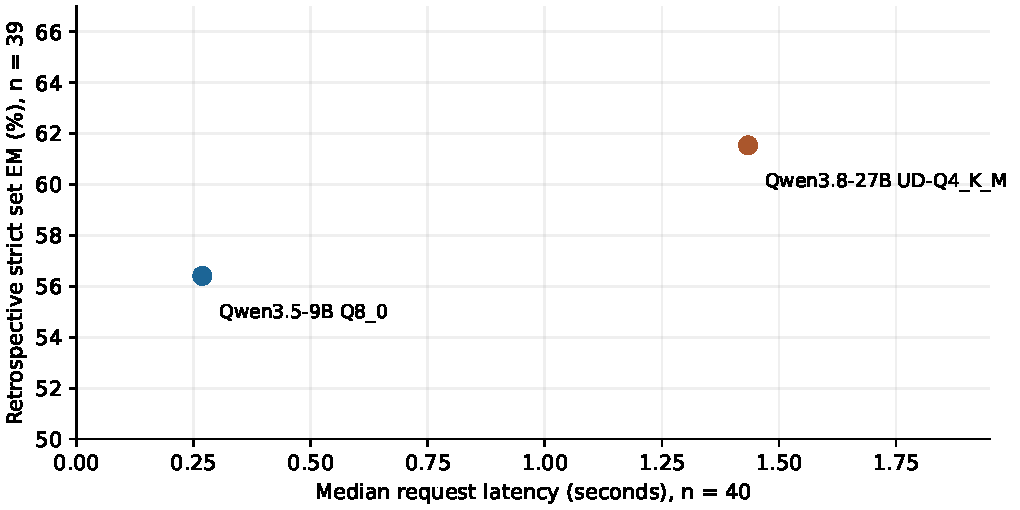
\includegraphics[width=\linewidth]{../results/20261004_article_build/native40_tradeoff.pdf}
\caption{Native TELEMETRY40: retrospective strict EM on 39 references versus measured request latency on 40 calls. These two practical configurations both reuse DEV; point values do not establish equivalence or a causal size effect.}\end{figure}

The initial native profile with 32 checkpoints produced RAM-censored Qwen27 attempts. A subsequent checkpoint-zero profile completed TELEMETRY40; all original failures remain archived. They were operational failures, not arithmetic errors. This repair and the absence of further errors establish behavior in the observed runs, not long-term reliability or reproducibility across machines.


\section{Calculations and completed tool execution}

Study C supplies a typed task name, question, public numeric inputs and explicit units to every arm. It evaluates simple daily growing-degree accumulation without an upper cap; saturation pressure and VPD; daily FAO-56 reference evapotranspiration; and the explicitly defined experimental gap max(0, target - sum(rain)). GDD sums max(0, (Tmin + Tmax)/2 - base) over the supplied days. Single-observation VPD uses saturation pressure times (1 - RH/100); the separate daily form uses temperature and humidity extrema. The rain gap is an arithmetic scenario, not an established field irrigation recommendation. FAO-56 ET0 is reference evapotranspiration rather than crop ETc or an irrigation dose \cite{ref19}. Missing quantities are not replaced by typical wind, zero soil heat flux, hidden reference values or crop thresholds.


The original 27-case study separates full answers, numbers and units, action correctness and declared tool IDs. Qwen9 and Qwen27 obtain full correctness 7/27 and 15/27; numeric correctness is 1/16 and 6/16. Correct tool declarations are 17/26 and 25/26, with the unsupported case excluded from that denominator. The deterministic executor attains 27/27 against the specified reference implementation and independently constructed formula gold. Replay using saved tool choices attains 17/26 and 25/26 by passing original inputs directly to code. Replay does not demonstrate that a model supplied valid arguments or completed a tool interaction. Qwen9 and Qwen27 historical responses also came from different checkpoint profiles, so their latency gap is not a matched model comparison.


The new predeclared live comparison completes all 108 model--arm decisions, with 140 measured model calls and two separate synthetic warmups. Both models use the checkpoint-zero native load/decoding profile. The model-only arm makes one call; the tool arm chooses an allowlisted tool and supplies its full argument objects, which are checked against the public request before execution. The application never completes arguments from gold, a hidden category or expected tool. A successful numeric execution is followed by a model finalization call. This is application-level JSON dispatch, with explicit typed task and contracts supplied; native provider function calling and unrestricted intent discovery were not evaluated.


\noindent\begin{minipage}{\linewidth}
Table 3. Matched development Study C, 27 cases per arm. Full correctness uses the preserved per-case value/action/tool scorer; final-schema compliance is audited separately. Latency is the median sum of model HTTP wall spans, excluding application dispatch and logging.


\begin{center}\begingroup\small\setlength{\tabcolsep}{4pt}
\begin{tabular}{@{}>{\raggedright\arraybackslash}p{0.28\linewidth}>{\raggedright\arraybackslash}p{0.16\linewidth}>{\raggedright\arraybackslash}p{0.16\linewidth}>{\raggedright\arraybackslash}p{0.16\linewidth}>{\raggedright\arraybackslash}p{0.14\linewidth}@{}}
\toprule
Configuration and arm & Full correct & Number + unit & Numeric executions & Summed latency, s \\
\midrule
Qwen9 model only & 7/27 & 1/16 & 0 & 1.469 \\
Qwen9 live tools & 18/27 & 16/16 & 16 & 2.857 \\
Qwen27 model only & 15/27 & 6/16 & 0 & 8.989 \\
Qwen27 live tools & 25/27 & 16/16 & 16 & 21.879 \\
\bottomrule\end{tabular}\endgroup\end{center}\end{minipage}

All 32 submitted numeric calls passed argument validation, executed the declared formula, and yielded correct final numeric values and units. Full nonnumeric correctness is 6/11 versus 2/11 for Qwen9 and 9/11 versus 9/11 for Qwen27, model-only versus tools. Thus the numeric improvement does not establish reliable clarification or unsupported-task handling; the smaller model loses correctness on four of those cases. No transport errors or output-budget truncations were observed. Offline JSON field-shape/type checks find Qwen9 compliant in 24/27 model-only and 26/27 tool outputs, and Qwen27 in 27/27 for both. Adding the allowed-tool-ID requirement gives Qwen9 22/27 and 19/27; Qwen27 remains at 27/27 in both arms. All four malformed field-type cases already fail the preserved full-answer scorer, so this separate contract check changes none of the table's correctness counts.


Each call allows at most 512 output tokens; a successful numeric tool interaction permits two calls and up to twice the aggregate generation budget. Tool feedback and the number of calls therefore change together. Reported latency sums the measured model requests, rather than the entire application's end-to-end time. The run is one matched development comparison on reused constructed material, not independent agronomic validation. Its weight sizes/paths match retained identity receipts; full weight SHA verification belongs to the earlier provenance receipt and was not repeated during timed inference.


Strict results retain the original per-case tolerances: 1e-8 for twelve high-precision constructed numerical cases, and 0.001, 0.005 or 0.01 for four published rounded controls. The separate rounding diagnostic uses max(original case tolerance, 1e-4), without replacing historical scores. These tolerances evaluate precision against the declared formula and instructions; they do not define farm-level acceptability. Rounded FAO worked examples and high-precision constructed references have different provenance. The original secondary diagnostic does not increase historical numeric correctness. Formula implementation checks cannot establish the suitability of inputs, crop decisions or agricultural deployment safety.


\section{Supplementary cloud observations and model coverage}

MERA DEV60 Mercury2.5 instant, 512-token outputs yield 31/59 strict matches, including four failed or truncated attempts. Saved-output escalation from Qwen9's 37/59 baseline does not improve EM over any retained nonzero threshold; its best retained threshold yields 35/59. Cloud-call fractions are simulated, and no live cascade latency or cost saving follows from that replay. Mercury is the historical direct cloud reference, with no claim to be the strongest cloud model.


OpenRouter's shared HOME DEV9 has nine completed outputs each for hosted Qwen3.8-27B, Ling3.0-Flash-Sante and Dots3-Note-Preview, scoring 5/9, 4/9 and 4/9 under the HOME scorer. These are supplementary API observations on a different dataset. Codex CLI's MERA DEV60 product/harness series has 36/59 strict matches with reasoning medium and 46 JSON presentation violations; one reference is unresolved. Claude Code's historical authentication probes produce no benchmark answers. Subscription latency includes process startup and harness overhead, and a subscription is not zero economic cost. Hosted display names do not establish local weight or serving identity.


Historical HOME150 tools-plus-cloud gives 139/150 and its local cascade 133/150. The cascade uses 20 rather than 100 cloud calls but fails its historical quality criterion. The separate Jev development series yields 30/36 versus rules 31/36, with total external requests 56 versus 23. These findings motivate transparent tool and request accounting; they do not provide an independent positive cloud-routing result for the present MERA comparison.


The repository coverage table identifies dataset, sample count, profile, completion, live/replay status and each model's role. The two optional checkpoints have separate bounded status records and are not required to complete the primary article.


\section{Limitations and reproducibility}

Public DEV was used repeatedly for compatibility, model selection and inspection. The 40-item telemetry subset reuses this data, and the calculation cases repeat specified formula families. Neither is an external confirmatory test. Differences in generation, architecture, quantization, decoding interface and GPU placement prevent a causal size interpretation. A single PC and sampled aggregate memory limit hardware generalization. Disabled reasoning and short output budgets limit the inference regime represented. Format violations, censored attempts and preserved configuration changes qualify the operational results.


The strict set scorer is reproducible locally, while MERA production scoring remains unresolved. Expert-created keys support the bounded benchmark evaluation without making the authors independent agronomic adjudicators. Benchmark licensing does not follow from the software license; restricted content and logs remain local. No learned router was trained on MERA material. Historical HOME claims remain bounded by their own synthetic and translation limitations.


The reproducibility package retains immutable historical runs, newly versioned analyses, prompt-byte and weight receipts, frozen protocols, per-attempt journals, load/warmup records and error counts. Raw restricted content is excluded from the editorial copy. Absent seed, actual GPU-layer count, exact per-model engine build and unobserved stop causes remain unknown. No new paid API spending, hidden TEST inference, submission, external contact or final license selection occurred in this session.


\section{Conclusions and disclosures}

The evaluated Qwen9 configuration offers lower occupied resources and shorter measured latency, while Qwen27 has higher observed strict quality. The full-split gap is descriptive evidence on selected DEV, and native subset outputs permit a narrower same-run quality--resource description. The comparison supports choosing a configuration according to an explicitly stated practical budget; it does not prove general superiority, equivalence or a pure parameter-count effect. Deterministic computation should be evaluated through actual arguments, validation, execution and a final answer, rather than a tool name alone.


Live deterministic execution improves specified numeric outcomes for both models, but Qwen9 retains tool-selection/clarification failures and successful interactions require an additional model call. Preparation of an English preprint and a Russian instructor-review version can continue without the pending MERA response. Any external submission still requires both authors' final review, publication metadata and rights decisions. The Russian and English versions describe one empirical study. Smaller released Qwen3.5 variants provide future deployment candidates; later generations can be evaluated under the same declared resource budget without assuming a future model name, release date or performance.


AI assistance was substantial: Codex agents supported literature checking, code, execution, analysis, visual preparation and manuscript drafting. This is AI review rather than completed human review. Antoniy Sarychev and Denis Shesternin remain the proposed human authors responsible for checking and approving the work. Contributions and final consent are pending human confirmation; no AI system or instructor is automatically an author. Software is Apache-2.0; manuscript licensing remains unselected and benchmark rights are separate.


\begin{thebibliography}{99}\small
\bibitem{ref1}Chen, L.; Zaharia, M.; Zou, J. \emph{FrugalGPT: How to Use Large Language Models While Reducing Cost and Improving Performance}. arXiv preprint, 2023. \href{https://arxiv.org/abs/2305.05176}{Primary source}.
\bibitem{ref2}Aggarwal, P.; Madaan, A.; Anand, A.; et al. \emph{AutoMix: Automatically Mixing Language Models}. arXiv preprint, 2023. \href{https://arxiv.org/abs/2310.12963}{Primary source}.
\bibitem{ref3}Ding, D.; Mallick, A.; Wang, C.; et al. \emph{Hybrid LLM: Cost-Efficient and Quality-Aware Query Routing}. arXiv preprint, 2024. \href{https://arxiv.org/abs/2404.14618}{Primary source}.
\bibitem{ref4}Ong, I.; Almahairi, A.; Wu, V.; et al. \emph{RouteLLM: Learning to Route LLMs from Preference Data}. ICLR 2025, 2025. \href{https://proceedings.iclr.cc/paper_files/paper/2025/hash/5503a7c69d48a2f86fc00b3dc09de686-Abstract-Conference.html}{Primary source}.
\bibitem{ref5}Dekoninck, J.; Baader, M.; Vechev, M. \emph{A Unified Approach to Routing and Cascading for LLMs}. ICML 2025, PMLR 267:12987-13010, 2025. \href{https://proceedings.mlr.press/v267/dekoninck25a.html}{Primary source}.
\bibitem{ref6}Hu, Q. J.; Bieker, J.; Li, X.; et al. \emph{RouterBench: A Benchmark for Multi-LLM Routing System}. arXiv preprint, 2024. \href{https://arxiv.org/abs/2403.12031}{Primary source}.
\bibitem{ref7}Kossen, J.; Han, J.; Razzak, M.; et al. \emph{Semantic Entropy Probes: Robust and Cheap Hallucination Detection in LLMs}. arXiv preprint, 2024. \href{https://arxiv.org/abs/2406.15927}{Primary source}.
\bibitem{ref8}Wen, B.; Yao, J.; Feng, S.; et al. \emph{Know Your Limits: A Survey of Abstention in Large Language Models}. arXiv preprint, 2024. \href{https://arxiv.org/abs/2407.18418}{Primary source}.
\bibitem{ref9}Yang, X.; Gao, J.; Xue, W.; et al. \emph{PLLaMa: An Open-source Large Language Model for Plant Science}. arXiv preprint, 2024. \href{https://arxiv.org/abs/2401.01600}{Primary source}.
\bibitem{ref10}Yang, B.; Zhang, Y.; Feng, L.; et al. \emph{AgriGPT: a Large Language Model Ecosystem for Agriculture}. arXiv preprint, 2025. \href{https://arxiv.org/abs/2508.08632}{Primary source}.
\bibitem{ref11}Samuel, D. J.; Skarga-Bandurova, I.; Sikolia, D.; et al. \emph{AgroLLM: Connecting Farmers and Agricultural Practices through Large Language Models for Enhanced Knowledge Transfer and Practical Application}. arXiv preprint, 2025. \href{https://arxiv.org/abs/2503.04788}{Primary source}.
\bibitem{ref12}Yang, B.; Zhang, Y.; Chen, Y.; et al. \emph{AgriAgent: Contract-Driven Planning and Capability-Aware Tool Orchestration in Real-World Agriculture}. arXiv preprint, 2026. \href{https://arxiv.org/abs/2601.08308}{Primary source}.
\bibitem{ref13}Ye, Z.; Wen, Y.; Fan, X.; et al. \emph{AgroTools: A Benchmark for Tool-Augmented Multimodal Agents in Agriculture}. arXiv preprint, 2026. \href{https://arxiv.org/abs/2605.22366}{Primary source}.
\bibitem{ref14}Yao, S.; Shinn, N.; Razavi, P.; et al. \emph{tau-bench: A Benchmark for Tool-Agent-User Interaction in Real-World Domains}. arXiv preprint, 2024. \href{https://arxiv.org/abs/2406.12045}{Primary source}.
\bibitem{ref15}Liu, W.; Huang, X.; Zeng, X.; et al. \emph{ToolACE: Winning the Points of LLM Function Calling}. ICLR 2025, 2025. \href{https://proceedings.iclr.cc/paper_files/paper/2025/hash/663865ea167425c6c562cb0b6bcf76c7-Abstract-Conference.html}{Primary source}.
\bibitem{ref16}Ma, S.; Wang, H.; Ma, L.; et al. \emph{The Era of 1-bit LLMs: All Large Language Models are in 1.58 Bits}. arXiv preprint, 2024. \href{https://arxiv.org/abs/2402.17764}{Primary source}.
\bibitem{ref17}Gemma Team; et al. \emph{Gemma 4 Technical Report}. arXiv preprint, 2026. \href{https://arxiv.org/abs/2607.02770}{Primary source}.
\bibitem{ref18}Kpodo, J.; Kordjamshidi, P.; Nejadhashemi, A. P. \emph{AgXQA: A benchmark for advanced Agricultural Extension question answering}. Computers and Electronics in Agriculture 225:109349, 2024. \href{https://doi.org/10.1016/j.compag.2024.109349}{Primary source}.
\bibitem{ref19}Allen, R. G.; Pereira, L. S.; Raes, D.; Smith, M. \emph{Crop evapotranspiration - Guidelines for computing crop water requirements}. FAO Irrigation and Drainage Paper 56, 1998. \href{https://www.fao.org/4/x0490e/x0490e00.htm}{Primary source}.
\end{thebibliography}
\end{document}
